\documentclass{beamer}
\usepackage[utf8]{inputenc}
\usepackage[T1]{fontenc}
\usepackage[russian]{babel}
\usepackage{graphicx}
\usepackage{listings}
\usepackage{amsmath, amssymb}

\usetheme{Madrid}
\setbeamertemplate{footline}[frame number]

\title{skip list}
\author{Кузьмищев Леонид}
\date{28.02.2026}

\begin{document}

\frame{\titlepage}

\begin{frame}{Skip list}
  Skip list — вероятностная структура данных, основанная на параллельных связных списках.

  \vspace{1em}

  \begin{itemize}
    \item Самый нижний уровень — обычный связный список, а каждый следующий список — подмножество предыдущего.
    \item Высота узла определяется посредством случайного эксперимента.
  \end{itemize}
\end{frame}

\begin{frame}{Пример}
  \begin{center}
    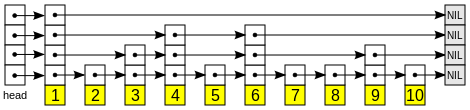
\includegraphics[width=0.8\textwidth]{image/Skip_list_example.png}
  \end{center}
\end{frame}

\begin{frame}{find}
    \begin{enumerate}
        \item Начинаем с головы списка и самого верхнего уровня
        \item Пока текущий уровень не ниже нуля:
        \begin{enumerate}
            \item На текущем уровне двигаемся вправо, пока следующий узел существует и его ключ меньше искомого
            \item Если следующий узел на этом уровне существует и его ключ равен искомому, возвращаем этот узел
            \item Спускаемся на уровень ниже
        \end{enumerate}
        \item Если элемент не найден, возвращаем NULL
    \end{enumerate}
\end{frame}

\begin{frame}{insert}
    \begin{enumerate}
        \item Создаём массив для хранения всех предшественников
        \item Находим место для вставки
        \item Случайно определяем высоту нового узла и добавляем его
        \item Перебрасываем указатели от $0$ до высоты узла
    \end{enumerate}
\end{frame}

\begin{frame}{delete}
    \begin{enumerate}
        \item Создаём массив для хранения всех предшественников
        \item Находим элемент и удаляем его
        \item Перебрасываем указатели от $0$ до высоты узла
    \end{enumerate}
\end{frame}

\begin{frame}{Асимптотика}
  \begin{center}
    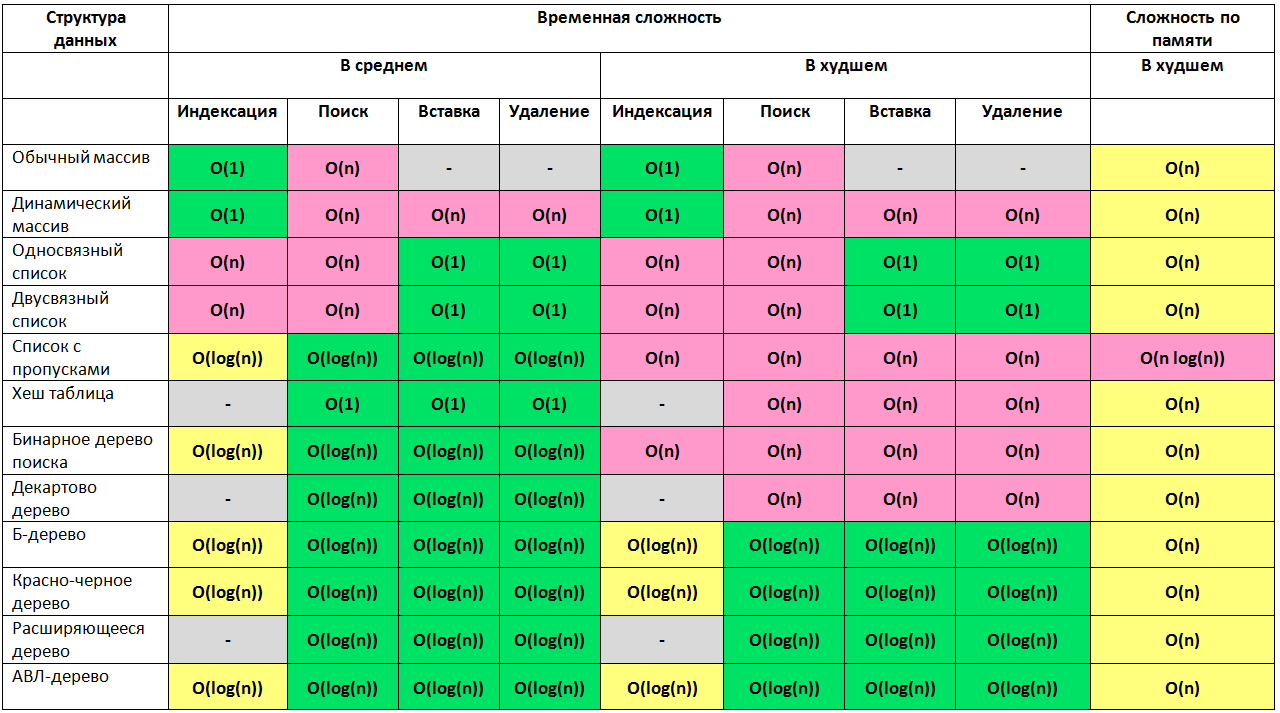
\includegraphics[width=0.8\textwidth]{image/asimptoty.png}
  \end{center}
\end{frame}

\begin{frame}{А почему не деревья?}
    \begin{itemize}
        \item говорят, что реализовать проще
            \item но однозачно проще отлаживать
        \item сценарии, в которых данные на входе сортированы и операций очень много
            \item константное время важно
            \item система логирования, например            
        \item легче адаптировать для параллельных алгоритмов
        \item деревья лучше 
    \end{itemize}
    ---
    \begin{itemize}
        \item реализация: https://github.com/leonilkuz-13/2sem$\_$homework$\_$repo/tree/skip$\_$list
    \end{itemize}
\end{frame}

\end{document}